\section{Background}
\label{chap:background}

\subsection{LUKS2 Disk Encryption}
\label{chap:background.luks2}
\emph{Linux Unified Key Setup 2}, or short LUKS2, is the second version of a disk encryption standard. It provides a specification \cite{Broz2018} for a on-disk format for storing the encryption metadata as well as the encrypted user data. Unlocking an encrypted disk is achieved by providing one of possibly multiple passphrases or keyfiles. The intended usage of LUKS2 is together with the Linux dm-crypt subsystem, but that is not mandatory\footnote{\label{fn:luks2windows} As we show in this thesis, it is possible to make the combination of LUKS2 and Windows work.}.

The differences between the original LUKS and LUKS2 are minor. According to \cite{Broz2018}, LUKS2 adds ``more flexible ways of storing metadata, redundant information to provide recovery in the case of corruption in a metadata area, and an interface to store externally managed metadata for integration with other tools.'' Practically, this means that LUKS2 has a different on-disk layout and, among other things, supports more password hashing algorithms (more precisely, password-based key derivation functions).

The reference implementation\footnote{\label{fn:background.luks2.referenceimpl} \url{https://gitlab.com/cryptsetup/cryptsetup}} is designed only for usage on Linux, which is why we developed a new Rust library for interacting with LUKS2 partitions. This is not a full equivalent, but only a cross-platform helper. Its task is to take care of all the cryptographic work needed before actually decrypting and encrypting data. Notably, it lacks the following features of the reference implementation:
\begin{itemize}[label=\textbf{--}]
	\item formatting new LUKS2 partitions,
	\item modifying or repairing existing LUKS2 partitions,
	\item converting a LUKS partition to a LUKS2 partition,
	\item actually mounting a LUKS2 partition for read/write usage (this is what our kernel driver and its userspace configuration tool is for).
\end{itemize}
Our library does provide access to the raw decrypted user data, but the practical use of this is very limited: the decrypted data is in the format of a filesystem, e.g. FAT32, btrfs, or Ext4. Therefore a filesystem driver is needed to actually access the stored files. One way of exposing the decrypted data to the system's filesystem drivers is by transparently decrypting the data directly in the kernel, which is what our driver does (see \autoref{chap:ourapproach}).

\subsubsection{On-Disk Format}
\label{chap:background.luks2.ondisk}
\begin{figure}[htb!]
	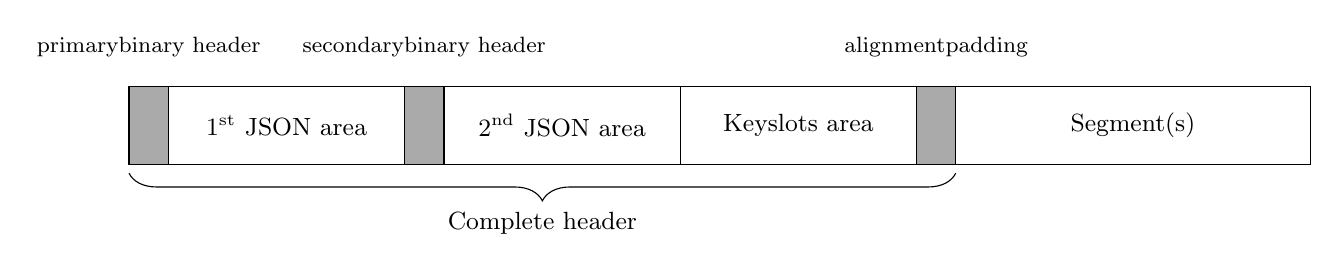
\begin{tikzpicture}
		\node [anchor=center] at (0.25, 1.5) {\footnotesize\makecell{primary\\binary header}};
		\draw [fill={rgb:black, 1; white, 2}] (0, 0) rectangle (0.5, 1);
		\draw [fill=white] (0.5, 0) rectangle (3.5, 1);
		\node [anchor=center] at (2, 0.5) {\small\makecell{1\textsuperscript{st} JSON area}};
		\node [anchor=center] at (3.75, 1.5) {\footnotesize\makecell{secondary\\binary header}};
		\draw [fill={rgb:black, 1; white, 2}] (3.5, 0) rectangle (4, 1);
		\draw [fill=white] (4, 0) rectangle (7, 1);
		\node [anchor=center] at (5.5, 0.5) {\small\makecell{2\textsuperscript{nd} JSON area}};
		\draw [fill=white] (7, 0) rectangle (10, 1);
		\node [anchor=center] at (8.5, 0.5) {\small\makecell{Keyslots area}};
		\node [anchor=center] at (10.25, 1.5) {\footnotesize\makecell{alignment\\padding}};
		\draw [fill={rgb:black, 1; white, 2}] (10, 0) rectangle (10.5, 1);

		\draw [decorate, decoration={brace, amplitude=10pt, mirror}, yshift=-3pt]
		(0, 0) -- (10.5, 0) node [black, midway, yshift=-18pt] {\small Complete header};

		\draw [fill=white] (10.5, 0) rectangle (15, 1);
		\node [anchor=center] at (12.75, 0.5) {\small\makecell{Segment(s)}};
	\end{tikzpicture}
	\caption[
		LUKS2 on-disk format
	]{
		LUKS2 on-disk format (modified after \cite{Broz2018}). The complete header consists of three areas: a binary header of exactly one 4096-byte sector, JSON metadata, and the binary keyslots data. A \emph{keyslot} is an ``encrypted area on disk that contains a key'' \cite{Broz2018}. For redundancy, the binary header and the JSON metadata are stored twice. After that follow one or areas containing encrypted user data. The specification calls these areas \emph{segments}.
	}
	\label{fig:background.luks2.ondisk}
\end{figure}

\autoref{fig:background.luks2.ondisk} shows the high-level layout of a LUKS2-encrypted disk.

The two binary headers have a size of exactly one sector, so that they are always written atomically. Only the first 512 bytes are actually used. The header marks the disk as following the LUKS2 specification, and contains metadata such as labels, a UUID, and a header checksum. The labels and UUID can be accessed using the \texttt{blkid}\footnote{\label{fn:background.luks2.blkid} \url{https://linux.die.net/man/8/blkid}} command-line tool and also be used in the \texttt{udev}\footnote{\label{fn:background.luks2.udev} \url{https://linux.die.net/man/8/udev}} Linux subsystem. For the detailed contents, see \autoref{fig:background.luks2.binhdrstructure}. \autoref{fig:background.luks2.binhdrexample} also contains an example hexdump of a binary header.

\begin{figure}[htb!]
	\begin{ccode}
#define MAGIC_1ST "LUKS\xba\xbe"
#define MAGIC_2ND "SKUL\xba\xbe"
#define MAGIC_L     6
#define UUID_L     40
#define LABEL_L    48
#define SALT_L     64
#define CSUM_ALG_L 32
#define CSUM_L     64

struct luks2_hdr_disk {
    char     magic[MAGIC_L];       // MAGIC_1ST or MAGIC_2ND
    uint16_t version;              // Version 2
    uint64_t hdr_size;             // size including JSON area [bytes]
    uint64_t seqid;                // sequence ID, increased on update
    char     label[LABEL_L];       // ASCII label or empty
    char     csum_alg[CSUM_ALG_L]; // checksum algorithm, "sha256"
    uint8_t  salt[SALT_L];         // salt, unique for every header
    char     uuid[UUID_L];         // UUID of device
    char     subsystem[LABEL_L];   // owner subsystem label or empty
    uint64_t hdr_offset;           // offset from device start [bytes]
    char    _padding[184];         // must be zeroed
    uint8_t  csum[CSUM_L];         // header checksum
    char    _padding4096[7*512];   // Padding, must be zeroed
} __attribute__((packed));
	\end{ccode}
	\caption[
		LUKS2 binary header structure
	]{
		LUKS2 binary header structure from \cite{Broz2018}. Integers are stored in big-endian format, and all strings have to be null-terminated. The \texttt{magic}, \texttt{version}, and \texttt{uuid} fields are also present in the LUKS1 binary header and were placed at the same offsets as there.
	}
	\label{fig:background.luks2.binhdrstructure}
\end{figure}

\begin{figure}[htb!]
	\ttfamily
	\scriptsize
	\begin{tabular}{c|*{16}{c}|l}
		0000 & \cellcolor{tPink}4C & \cellcolor{tPink}55 & \cellcolor{tPink}4B & \cellcolor{tPink}53 & \cellcolor{tPink}BA & \cellcolor{tPink}BE & \cellcolor{tOrng}00 & \cellcolor{tOrng}02 & \cellcolor{tYlow}00 & \cellcolor{tYlow}00 & \cellcolor{tYlow}00 & \cellcolor{tYlow}00 & \cellcolor{tYlow}00 & \cellcolor{tYlow}00 & \cellcolor{tYlow}40 & \cellcolor{tYlow}00 & \coltxt{tPink}{LUKSº¾}\coltxt{tOrng}{..}\coltxt{tYlow}{......@.} \\
		0010 & \cellcolor{tGren}00 & \cellcolor{tGren}00 & \cellcolor{tGren}00 & \cellcolor{tGren}00 & \cellcolor{tGren}00 & \cellcolor{tGren}00 & \cellcolor{tGren}00 & \cellcolor{tGren}03 & \cellcolor{tLblu}54 & \cellcolor{tLblu}68 & \cellcolor{tLblu}69 & \cellcolor{tLblu}73 & \cellcolor{tLblu}20 & \cellcolor{tLblu}69 & \cellcolor{tLblu}73 & \cellcolor{tLblu}20 & \coltxt{tGren}{........}\coltxt{tLblu}{This is } \\
		0020 & \cellcolor{tLblu}61 & \cellcolor{tLblu}6E & \cellcolor{tLblu}20 & \cellcolor{tLblu}41 & \cellcolor{tLblu}53 & \cellcolor{tLblu}43 & \cellcolor{tLblu}49 & \cellcolor{tLblu}49 & \cellcolor{tLblu}20 & \cellcolor{tLblu}6C & \cellcolor{tLblu}61 & \cellcolor{tLblu}62 & \cellcolor{tLblu}65 & \cellcolor{tLblu}6C & \cellcolor{tLblu}00 & \cellcolor{tLblu}00 & \coltxt{tLblu}{an ASCII label..} \\
		0030 & \cellcolor{tLblu}00 & \cellcolor{tLblu}00 & \cellcolor{tLblu}00 & \cellcolor{tLblu}00 & \cellcolor{tLblu}00 & \cellcolor{tLblu}00 & \cellcolor{tLblu}00 & \cellcolor{tLblu}00 & \cellcolor{tLblu}00 & \cellcolor{tLblu}00 & \cellcolor{tLblu}00 & \cellcolor{tLblu}00 & \cellcolor{tLblu}00 & \cellcolor{tLblu}00 & \cellcolor{tLblu}00 & \cellcolor{tLblu}00 & \coltxt{tLblu}{................} \\
		0040 & \cellcolor{tLblu}00 & \cellcolor{tLblu}00 & \cellcolor{tLblu}00 & \cellcolor{tLblu}00 & \cellcolor{tLblu}00 & \cellcolor{tLblu}00 & \cellcolor{tLblu}00 & \cellcolor{tLblu}00 & \cellcolor{tBlue}73 & \cellcolor{tBlue}68 & \cellcolor{tBlue}61 & \cellcolor{tBlue}32 & \cellcolor{tBlue}35 & \cellcolor{tBlue}36 & \cellcolor{tBlue}00 & \cellcolor{tBlue}00 & \coltxt{tLblu}{........}\coltxt{tBlue}{sha256..} \\
		0050 & \cellcolor{tBlue}00 & \cellcolor{tBlue}00 & \cellcolor{tBlue}00 & \cellcolor{tBlue}00 & \cellcolor{tBlue}00 & \cellcolor{tBlue}00 & \cellcolor{tBlue}00 & \cellcolor{tBlue}00 & \cellcolor{tBlue}00 & \cellcolor{tBlue}00 & \cellcolor{tBlue}00 & \cellcolor{tBlue}00 & \cellcolor{tBlue}00 & \cellcolor{tBlue}00 & \cellcolor{tBlue}00 & \cellcolor{tBlue}00 & \coltxt{tBlue}{................} \\
		0060 & \cellcolor{tBlue}00 & \cellcolor{tBlue}00 & \cellcolor{tBlue}00 & \cellcolor{tBlue}00 & \cellcolor{tBlue}00 & \cellcolor{tBlue}00 & \cellcolor{tBlue}00 & \cellcolor{tBlue}00 & \cellcolor{tPurp}EB & \cellcolor{tPurp}0F & \cellcolor{tPurp}D2 & \cellcolor{tPurp}C6 & \cellcolor{tPurp}E3 & \cellcolor{tPurp}D2 & \cellcolor{tPurp}8D & \cellcolor{tPurp}4B & \coltxt{tBlue}{........}\coltxt{tPurp}{ë.ÒÆãÒ.K} \\
		0070 & \cellcolor{tPurp}BB & \cellcolor{tPurp}2B & \cellcolor{tPurp}8A & \cellcolor{tPurp}49 & \cellcolor{tPurp}E6 & \cellcolor{tPurp}2E & \cellcolor{tPurp}4E & \cellcolor{tPurp}B7 & \cellcolor{tPurp}04 & \cellcolor{tPurp}2F & \cellcolor{tPurp}A9 & \cellcolor{tPurp}39 & \cellcolor{tPurp}76 & \cellcolor{tPurp}71 & \cellcolor{tPurp}8F & \cellcolor{tPurp}8A & \coltxt{tPurp}{»+ŠIæ.N·./©9vq.Š} \\
		0080 & \cellcolor{tPurp}33 & \cellcolor{tPurp}E8 & \cellcolor{tPurp}F3 & \cellcolor{tPurp}90 & \cellcolor{tPurp}FF & \cellcolor{tPurp}DC & \cellcolor{tPurp}4D & \cellcolor{tPurp}3D & \cellcolor{tPurp}E8 & \cellcolor{tPurp}30 & \cellcolor{tPurp}7B & \cellcolor{tPurp}37 & \cellcolor{tPurp}01 & \cellcolor{tPurp}30 & \cellcolor{tPurp}E7 & \cellcolor{tPurp}5D & \coltxt{tPurp}{3èó.ÿÜM=è0\{7.0ç]} \\
		0090 & \cellcolor{tPurp}AD & \cellcolor{tPurp}A0 & \cellcolor{tPurp}57 & \cellcolor{tPurp}1C & \cellcolor{tPurp}0E & \cellcolor{tPurp}63 & \cellcolor{tPurp}BC & \cellcolor{tPurp}D4 & \cellcolor{tPurp}DD & \cellcolor{tPurp}3C & \cellcolor{tPurp}EC & \cellcolor{tPurp}F5 & \cellcolor{tPurp}DE & \cellcolor{tPurp}67 & \cellcolor{tPurp}F8 & \cellcolor{tPurp}D8 & \coltxt{tPurp}{..W..c¼ÔÝ<ìõÞgøØ} \\
		00A0 & \cellcolor{tPurp}F2 & \cellcolor{tPurp}7E & \cellcolor{tPurp}82 & \cellcolor{tPurp}CD & \cellcolor{tPurp}B9 & \cellcolor{tPurp}DD & \cellcolor{tPurp}77 & \cellcolor{tPurp}10 & \cellcolor{tRose}65 & \cellcolor{tRose}39 & \cellcolor{tRose}33 & \cellcolor{tRose}64 & \cellcolor{tRose}63 & \cellcolor{tRose}61 & \cellcolor{tRose}66 & \cellcolor{tRose}61 & \coltxt{tPurp}{ò\nicetilde{}‚͹Ýw.}\coltxt{tRose}{e93dcafa} \\
		00B0 & \cellcolor{tRose}2D & \cellcolor{tRose}65 & \cellcolor{tRose}65 & \cellcolor{tRose}30 & \cellcolor{tRose}62 & \cellcolor{tRose}2D & \cellcolor{tRose}34 & \cellcolor{tRose}31 & \cellcolor{tRose}36 & \cellcolor{tRose}38 & \cellcolor{tRose}2D & \cellcolor{tRose}61 & \cellcolor{tRose}61 & \cellcolor{tRose}37 & \cellcolor{tRose}63 & \cellcolor{tRose}2D & \coltxt{tRose}{-ee0b-4168-aa7c-} \\
		00C0 & \cellcolor{tRose}66 & \cellcolor{tRose}33 & \cellcolor{tRose}30 & \cellcolor{tRose}34 & \cellcolor{tRose}37 & \cellcolor{tRose}34 & \cellcolor{tRose}38 & \cellcolor{tRose}38 & \cellcolor{tRose}36 & \cellcolor{tRose}61 & \cellcolor{tRose}32 & \cellcolor{tRose}65 & \cellcolor{tRose}00 & \cellcolor{tRose}00 & \cellcolor{tRose}00 & \cellcolor{tRose}00 & \coltxt{tRose}{f30474886a2e....} \\
		00D0 & \cellcolor{tPink}54 & \cellcolor{tPink}68 & \cellcolor{tPink}69 & \cellcolor{tPink}73 & \cellcolor{tPink}20 & \cellcolor{tPink}69 & \cellcolor{tPink}73 & \cellcolor{tPink}20 & \cellcolor{tPink}61 & \cellcolor{tPink}6E & \cellcolor{tPink}20 & \cellcolor{tPink}6F & \cellcolor{tPink}70 & \cellcolor{tPink}74 & \cellcolor{tPink}69 & \cellcolor{tPink}6F & \coltxt{tPink}{This is an optio} \\
		00E0 & \cellcolor{tPink}6E & \cellcolor{tPink}61 & \cellcolor{tPink}6C & \cellcolor{tPink}20 & \cellcolor{tPink}73 & \cellcolor{tPink}65 & \cellcolor{tPink}63 & \cellcolor{tPink}6F & \cellcolor{tPink}6E & \cellcolor{tPink}64 & \cellcolor{tPink}61 & \cellcolor{tPink}72 & \cellcolor{tPink}79 & \cellcolor{tPink}20 & \cellcolor{tPink}6C & \cellcolor{tPink}61 & \coltxt{tPink}{nal secondary la} \\
		00F0 & \cellcolor{tPink}62 & \cellcolor{tPink}65 & \cellcolor{tPink}6C & \cellcolor{tPink}00 & \cellcolor{tPink}00 & \cellcolor{tPink}00 & \cellcolor{tPink}00 & \cellcolor{tPink}00 & \cellcolor{tPink}00 & \cellcolor{tPink}00 & \cellcolor{tPink}00 & \cellcolor{tPink}00 & \cellcolor{tPink}00 & \cellcolor{tPink}00 & \cellcolor{tPink}00 & \cellcolor{tPink}00 & \coltxt{tPink}{bel.............} \\
		0100 & \cellcolor{tOrng}00 & \cellcolor{tOrng}00 & \cellcolor{tOrng}00 & \cellcolor{tOrng}00 & \cellcolor{tOrng}00 & \cellcolor{tOrng}00 & \cellcolor{tOrng}00 & \cellcolor{tOrng}00 & \cellcolor{tYlow}00 & \cellcolor{tYlow}00 & \cellcolor{tYlow}00 & \cellcolor{tYlow}00 & \cellcolor{tYlow}00 & \cellcolor{tYlow}00 & \cellcolor{tYlow}00 & \cellcolor{tYlow}00 & \coltxt{tOrng}{........}\coltxt{tYlow}{........} \\
		0110 & \cellcolor{tYlow}00 & \cellcolor{tYlow}00 & \cellcolor{tYlow}00 & \cellcolor{tYlow}00 & \cellcolor{tYlow}00 & \cellcolor{tYlow}00 & \cellcolor{tYlow}00 & \cellcolor{tYlow}00 & \cellcolor{tYlow}00 & \cellcolor{tYlow}00 & \cellcolor{tYlow}00 & \cellcolor{tYlow}00 & \cellcolor{tYlow}00 & \cellcolor{tYlow}00 & \cellcolor{tYlow}00 & \cellcolor{tYlow}00 & \coltxt{tYlow}{................} \\
		0120 & \cellcolor{tYlow}00 & \cellcolor{tYlow}00 & \cellcolor{tYlow}00 & \cellcolor{tYlow}00 & \cellcolor{tYlow}00 & \cellcolor{tYlow}00 & \cellcolor{tYlow}00 & \cellcolor{tYlow}00 & \cellcolor{tYlow}00 & \cellcolor{tYlow}00 & \cellcolor{tYlow}00 & \cellcolor{tYlow}00 & \cellcolor{tYlow}00 & \cellcolor{tYlow}00 & \cellcolor{tYlow}00 & \cellcolor{tYlow}00 & \coltxt{tYlow}{................} \\
		0130 & \cellcolor{tYlow}00 & \cellcolor{tYlow}00 & \cellcolor{tYlow}00 & \cellcolor{tYlow}00 & \cellcolor{tYlow}00 & \cellcolor{tYlow}00 & \cellcolor{tYlow}00 & \cellcolor{tYlow}00 & \cellcolor{tYlow}00 & \cellcolor{tYlow}00 & \cellcolor{tYlow}00 & \cellcolor{tYlow}00 & \cellcolor{tYlow}00 & \cellcolor{tYlow}00 & \cellcolor{tYlow}00 & \cellcolor{tYlow}00 & \coltxt{tYlow}{................} \\
		0140 & \cellcolor{tYlow}00 & \cellcolor{tYlow}00 & \cellcolor{tYlow}00 & \cellcolor{tYlow}00 & \cellcolor{tYlow}00 & \cellcolor{tYlow}00 & \cellcolor{tYlow}00 & \cellcolor{tYlow}00 & \cellcolor{tYlow}00 & \cellcolor{tYlow}00 & \cellcolor{tYlow}00 & \cellcolor{tYlow}00 & \cellcolor{tYlow}00 & \cellcolor{tYlow}00 & \cellcolor{tYlow}00 & \cellcolor{tYlow}00 & \coltxt{tYlow}{................} \\
		0150 & \cellcolor{tYlow}00 & \cellcolor{tYlow}00 & \cellcolor{tYlow}00 & \cellcolor{tYlow}00 & \cellcolor{tYlow}00 & \cellcolor{tYlow}00 & \cellcolor{tYlow}00 & \cellcolor{tYlow}00 & \cellcolor{tYlow}00 & \cellcolor{tYlow}00 & \cellcolor{tYlow}00 & \cellcolor{tYlow}00 & \cellcolor{tYlow}00 & \cellcolor{tYlow}00 & \cellcolor{tYlow}00 & \cellcolor{tYlow}00 & \coltxt{tYlow}{................} \\
		0160 & \cellcolor{tYlow}00 & \cellcolor{tYlow}00 & \cellcolor{tYlow}00 & \cellcolor{tYlow}00 & \cellcolor{tYlow}00 & \cellcolor{tYlow}00 & \cellcolor{tYlow}00 & \cellcolor{tYlow}00 & \cellcolor{tYlow}00 & \cellcolor{tYlow}00 & \cellcolor{tYlow}00 & \cellcolor{tYlow}00 & \cellcolor{tYlow}00 & \cellcolor{tYlow}00 & \cellcolor{tYlow}00 & \cellcolor{tYlow}00 & \coltxt{tYlow}{................} \\
		0170 & \cellcolor{tYlow}00 & \cellcolor{tYlow}00 & \cellcolor{tYlow}00 & \cellcolor{tYlow}00 & \cellcolor{tYlow}00 & \cellcolor{tYlow}00 & \cellcolor{tYlow}00 & \cellcolor{tYlow}00 & \cellcolor{tYlow}00 & \cellcolor{tYlow}00 & \cellcolor{tYlow}00 & \cellcolor{tYlow}00 & \cellcolor{tYlow}00 & \cellcolor{tYlow}00 & \cellcolor{tYlow}00 & \cellcolor{tYlow}00 & \coltxt{tYlow}{................} \\
		0180 & \cellcolor{tYlow}00 & \cellcolor{tYlow}00 & \cellcolor{tYlow}00 & \cellcolor{tYlow}00 & \cellcolor{tYlow}00 & \cellcolor{tYlow}00 & \cellcolor{tYlow}00 & \cellcolor{tYlow}00 & \cellcolor{tYlow}00 & \cellcolor{tYlow}00 & \cellcolor{tYlow}00 & \cellcolor{tYlow}00 & \cellcolor{tYlow}00 & \cellcolor{tYlow}00 & \cellcolor{tYlow}00 & \cellcolor{tYlow}00 & \coltxt{tYlow}{................} \\
		0190 & \cellcolor{tYlow}00 & \cellcolor{tYlow}00 & \cellcolor{tYlow}00 & \cellcolor{tYlow}00 & \cellcolor{tYlow}00 & \cellcolor{tYlow}00 & \cellcolor{tYlow}00 & \cellcolor{tYlow}00 & \cellcolor{tYlow}00 & \cellcolor{tYlow}00 & \cellcolor{tYlow}00 & \cellcolor{tYlow}00 & \cellcolor{tYlow}00 & \cellcolor{tYlow}00 & \cellcolor{tYlow}00 & \cellcolor{tYlow}00 & \coltxt{tYlow}{................} \\
		01A0 & \cellcolor{tYlow}00 & \cellcolor{tYlow}00 & \cellcolor{tYlow}00 & \cellcolor{tYlow}00 & \cellcolor{tYlow}00 & \cellcolor{tYlow}00 & \cellcolor{tYlow}00 & \cellcolor{tYlow}00 & \cellcolor{tYlow}00 & \cellcolor{tYlow}00 & \cellcolor{tYlow}00 & \cellcolor{tYlow}00 & \cellcolor{tYlow}00 & \cellcolor{tYlow}00 & \cellcolor{tYlow}00 & \cellcolor{tYlow}00 & \coltxt{tYlow}{................} \\
		01B0 & \cellcolor{tYlow}00 & \cellcolor{tYlow}00 & \cellcolor{tYlow}00 & \cellcolor{tYlow}00 & \cellcolor{tYlow}00 & \cellcolor{tYlow}00 & \cellcolor{tYlow}00 & \cellcolor{tYlow}00 & \cellcolor{tYlow}00 & \cellcolor{tYlow}00 & \cellcolor{tYlow}00 & \cellcolor{tYlow}00 & \cellcolor{tYlow}00 & \cellcolor{tYlow}00 & \cellcolor{tYlow}00 & \cellcolor{tYlow}00 & \coltxt{tYlow}{................} \\
		01C0 & \cellcolor{tGren}91 & \cellcolor{tGren}A4 & \cellcolor{tGren}A9 & \cellcolor{tGren}83 & \cellcolor{tGren}03 & \cellcolor{tGren}FF & \cellcolor{tGren}FB & \cellcolor{tGren}68 & \cellcolor{tGren}4E & \cellcolor{tGren}C2 & \cellcolor{tGren}94 & \cellcolor{tGren}6F & \cellcolor{tGren}4C & \cellcolor{tGren}78 & \cellcolor{tGren}71 & \cellcolor{tGren}AF & \coltxt{tGren}{‘¤©ƒ.ÿûhN”oLxq¯} \\
		01D0 & \cellcolor{tGren}AE & \cellcolor{tGren}1A & \cellcolor{tGren}91 & \cellcolor{tGren}F8 & \cellcolor{tGren}E0 & \cellcolor{tGren}2C & \cellcolor{tGren}F3 & \cellcolor{tGren}71 & \cellcolor{tGren}D5 & \cellcolor{tGren}17 & \cellcolor{tGren}CB & \cellcolor{tGren}60 & \cellcolor{tGren}E5 & \cellcolor{tGren}2F & \cellcolor{tGren}D6 & \cellcolor{tGren}36 & \coltxt{tGren}{®.‘øà,óqÕ.Ë`å/Ö6} \\
		01E0 & \cellcolor{tGren}00 & \cellcolor{tGren}00 & \cellcolor{tGren}00 & \cellcolor{tGren}00 & \cellcolor{tGren}00 & \cellcolor{tGren}00 & \cellcolor{tGren}00 & \cellcolor{tGren}00 & \cellcolor{tGren}00 & \cellcolor{tGren}00 & \cellcolor{tGren}00 & \cellcolor{tGren}00 & \cellcolor{tGren}00 & \cellcolor{tGren}00 & \cellcolor{tGren}00 & \cellcolor{tGren}00 & \coltxt{tGren}{................} \\
		01F0 & \cellcolor{tGren}00 & \cellcolor{tGren}00 & \cellcolor{tGren}00 & \cellcolor{tGren}00 & \cellcolor{tGren}00 & \cellcolor{tGren}00 & \cellcolor{tGren}00 & \cellcolor{tGren}00 & \cellcolor{tGren}00 & \cellcolor{tGren}00 & \cellcolor{tGren}00 & \cellcolor{tGren}00 & \cellcolor{tGren}00 & \cellcolor{tGren}00 & \cellcolor{tGren}00 & \cellcolor{tGren}00 & \coltxt{tGren}{................}
	\end{tabular}
	\caption[
		LUKS2 binary header example
	]{
		LUKS2 binary header example. The fields, as described in \autoref{fig:background.luks2.binhdrstructure}, were coloured differently to be easily distinguishable. A similar header, although with different salt and hash, can be generated by executing \texttt{fallocate -l 16M luks2.img \&\& cryptsetup luksFormat ---label 'This is an ASCII label' ---subsystem 'This is an optional secondary label' ---uuid e93dcafa-ee0b-4168-aa7c-f30474886a2e luks2.img} in a Linux shell.
	}
	\label{fig:background.luks2.binhdrexample}
\end{figure}

The sector containing the binary header is followed by the JSON area. This area arguably contains the metadata that is most relevant for decryption and encryption. \autoref{fig:background.luks2.jsonobjects} contains an overview of the objects stored in JSON and their relationships. For this thesis' brevity's sake, please refer to Chapter 3.1 in \cite{Broz2018} for an example of a LUKS2 JSON area.

\begin{figure}[htb!]
	\center
	\begin{tikzpicture}
		\node       (pass) at (4, 3.5)  {\small Passphrase};
		\node       (stor) at (8, 3.5)  {\small External Keystore};
		\node[rect] (dgst) at (0, 1.75) {\small Digest};
		\node[rect] (kslt) at (4, 1.75) {\small Keyslot};
		\node[rect] (tokn) at (8, 1.75) {\small Token};
		\node[rect] (conf) at (0, 0)    {\small Config};
		\node[rect] (segm) at (4, 0)    {\small Segment};

		\draw (pass) edge[arrow] (kslt);
		\draw (stor) edge[arrow] (tokn);

		\draw (dgst) edge[arrow] node[anchor=south, yshift=-4pt] {\small\makecell{validates}}   (kslt);
		\draw (tokn) edge[arrow] node[anchor=south, yshift=-4pt] {\small\makecell{can open}}    (kslt);
		\draw (kslt) edge[arrow] node[anchor=west]               {\small\makecell{is used for}} (segm);
	\end{tikzpicture}
	\caption[
		LUKS2 object schema
	]{
		LUKS2 object schema from \cite{Broz2018}. The most important objects are the following: \emph{keyslots}, which describe the details of how cryptographic keys are stored and encrypted; \emph{digests}, which can be used to verify that one has successfully extracted a key from a keyslot; and \emph{segments}, which describe the disk areas where the encrypted user data is stored. \autoref{fig:background.luks2.ondisk} shows where the areas described by the keyslot and segment objects actually lie on disk.
	}
	\label{fig:background.luks2.jsonobjects}
\end{figure}

After the JSON area, the keyslots area is stored on the disk. This is space reserved for storing encrypted cryptographic keys. The metadata from the JSON keyslot objects describe the position of a key on the disk as well as information on how to decrypt it. 

\subsubsection{Unlocking a Partition}
\label{chap:background.luks2.unlocking}
For simplicity, our LUKS2 Rust library does not support unlocking a keyslot using an external keystore defined by a token. Only unlocking via password is implemented. The library does however include support for different \emph{password-based key derivation functions (PBKDFs)}, namely \texttt{pbkdf2} with SHA-256, \texttt{argon2i}, and \texttt{argon2id}. These are all the PBKDF algorithms that are listed in the LUKS2 specification (see \cite{Broz2018}, Table 3). The default PBKDF used by LUKS2 is \texttt{argon2i} \cite{Cryptsetup2020}.

The LUKS2 specification allows for multiple segments in one partition. To make things easier, our driver only supports unlocking one segment. Therefore, in this thesis we may speak of unlocking a partition and mean unlocking one of the partition's segments.

To unlock a segment means to derive the cryptographic key that is needed for reading decrypted or writing encrypted data. This key is called the segment's \emph{master key}.

LUKS2 uses a process called \emph{anti-forensic splitting} to store the master key on the disk. This method was introduced in \cite{Fruhwirth2005}. It is used to diffuse the key's bytes into a longer sequence of bytes that has the following property: if at least one bit of the diffused sequence is changed, the key cannot be recovered. This is achieved by a clever combination of XOR and a hash function. The motivation behind this to make it easier (or possible) to dispose of an old key in such a way that it cannot be recovered from the disk. This is because it is much more feasible to partially erase a long sequence of bytes than to completely erase a short sequence. Erasing here means to overwrite the data in such a way that it cannot be recovered, which is not as trivial as one might think.

\cite{Fruhwirth2005} calls the operation that splits data anti-forensically AFsplit and the recovery operation AFmerge. We will adhere to this convention (with slight variations).

To necessitate the need of a password to recover the key, the data is also encrypted before it gets written to the disk. The encryption key is a hash of the password obtained by a PBKDF.

The properties of anti-forensic splitting can be used when the user wants to change the password: the master key is derived using the old password and then re-encrypted with the new password. The key as it was encrypted with the old password can then be destroyed.

\cite{Fruhwirth2005} presents two templates for storing keys, TKS1 and TKS2. The difference is whether the key is encrypted before or after splitting it. LUKS and LUKS2 use TKS2, which is schematically explained in \autoref{fig:background.luks2.tks2}. The hash function used by LUKS2 for anti-forensic splitting is SHA-256. \autoref{fig:background.luks2.masterkeydecrypt} shows the outline of an implementation of TKS2 in Rust.

\begin{figure}[htb!]
	\center
	\begin{tikzpicture}
		\node[rect, anchor=east] (pbkdf) at (8, 4) {\small PBKDF2};
		\node[rect]              (ciphr) at (3, 2) {\small Cipher};
		\node[rect, anchor=west] (merge) at (8, 2) {\small AF-merge};
		\node[rect, anchor=east] (rtcip) at (8, -0.5) {\small Real time cipher};

		\draw[arrow] (ciphr)                   -- node[anchor=south, yshift=-4pt] {\small\makecell{Split master key}}  (merge);
		\draw[arrow] (pbkdf.west)  + (-2.5, 0) -- node[anchor=south, yshift=-4pt] {\small\makecell{Passphrase}}          (pbkdf.west);
		\draw[arrow] (pbkdf.north) + (-0.6, 1) -- node[anchor=west]               {\small\makecell{Salt}}                +(-0.6, 0);
		\draw[arrow] (pbkdf.north) + (0.6,  1) -- node[anchor=west]               {\small\makecell{Hash iteration rate}} +(0.6,  0);
		\draw[arrow] (ciphr.west)  + (-2.5, 0) -- node[anchor=south, yshift=-4pt] {\small\makecell{Key storage}}         (ciphr.west);
		\draw[arrow] (rtcip.west)  + (-4,   0) -- node[anchor=south, yshift=-4pt] {\small\makecell{Encrypted partition}} (rtcip.west);
		\draw[arrow] (rtcip.east)              -- node[anchor=south, yshift=-4pt] {\small\makecell{Recovered partition}} +(4,    0);

		\draw[arrow] (pbkdf.east) -- +(1, 0) -- +(1, -1) -| (ciphr.north);
		\draw[arrow] (merge.east) -- +(1, 0) -- +(1, -1) -| node[anchor=east, yshift=-1.2em] {\small\makecell{Master key}} (rtcip.north);
	\end{tikzpicture}
	\caption[
		TKS2 scheme
	]{
		TKS2 scheme (modified after \cite{Fruhwirth2005}).
	}
	\label{fig:background.luks2.tks2}
\end{figure}

\begin{figure}[htb!]
	\begin{rustcode}
fn decrypt_keyslot(
	password: &[u8], keyslot: &LuksKeyslot, json: &LuksJson, /* ... */
) -> Result<Vec<u8>, LuksError> {
	let mut k = vec![
		0; keyslot.key_size() as usize * keyslot.af.stripes() as usize
	];
	// read keyslot data from disk into k...

	let mut pw_hash = vec![0; area.key_size() as usize];
	match keyslot.kdf() {
		// hash into pw_hash using pbkdf2, argon2i, or argon2id...
	}

	// decrypt keyslot area using the password hash as key
	match area.key_size() {
		32 => {
			let key1 = Aes128::new_varkey(&pw_hash[..16]).unwrap();
			let key2 = Aes128::new_varkey(&pw_hash[16..]).unwrap();
			let xts = Xts128::<Aes128>::new(key1, key2);
			xts.decrypt_area(&mut k, sector_size, 0, get_tweak_default);
		},
		// 64 byte key uses AES256 instead...
	}

	// merge and hash master key
	let master_key = af::merge(
		&k, keyslot.key_size() as usize, af.stripes() as usize
	);
	let digest_actual = base64::decode(json.digests[&0].digest())?;
	let mut digest_computed = vec![0; digest_actual.len()];
	let salt = base64::decode(json.digests[&0].salt())?;
	pbkdf2::pbkdf2::<Hmac<Sha256>>(
		&master_key, &salt, json.digests[&0].iterations(), &mut digest_computed
	);

	// compare digests
	if digest_computed == digest_actual {
		Ok(master_key)
	} else {
		Err(LuksError::InvalidPassword)
	}
}
	\end{rustcode}
	\caption[
		LUKS2 master key decryption in Rust
	]{
		LUKS2 master key decryption in Rust. Some values are hardcoded: only the digest with index 0 is used (lines 29, 31, 33), and it is assumed that the digest algorithm is always \texttt{pbkdf2} with SHA-256 (line 32). The latter is compliant with the specification, which lists this digest algorithm as the only option, but not optimal in the sense of input validation.
	}
	\label{fig:background.luks2.masterkeydecrypt}
\end{figure}

The keyslots area on the disk is large enough to store multiple split and encrypted master keys. Thus one can configure a LUKS2 partition to be unlocked by different passwords. Unlocking then works as described in \autoref{fig:background.luks2.unlocking}.

\begin{figure}[htb!]
	\center
	\begin{mdframed}
		\begin{enumerate}
			\item The user supplies a password.
			\item One of the available keyslots is selected.
			\item Using the password and keyslot, the master key is decrypted as described above.
			\item The derived master key is hashed and the result compared to the corresponding digest. Which digest and what hash parameters to used is defined in the JSON section.
			\item If the digests match, the master key has been successfully decrypted. Else go to step 2 and select a keyslot that has not been used yet.
			\item If the master key could not be decrypted with all available keyslots, the supplied password was not correct.
		\end{enumerate}
	\end{mdframed}
	\caption[
		LUKS2 master key decryption with multiple available keyslots
	]{
		LUKS2 master key decryption with multiple available keyslots. LUKS2 allows defining priorities that govern the order in that the available keyslots are tried. For a more detailed pseudocode see Figure 5 in \cite{Fruwirth2018}.
	}
	\label{fig:background.luks2.unlocking}
\end{figure}

\subsubsection{Using an Unlocked Partition}
\label{chap:background.luks2.using}
After a partition has been unlocked, i.e. after the master key of one of its segments has been decrypted, the partition is ready to be read from and written to. This happens using what \autoref{fig:background.luks2.tks2} calls a real time cipher. LUKS2 supports different encryption algorithms for this purpose, see \autoref{fig:background.luks2.encryptionalgorithms} for a selection of them. Our driver only supports the default aes-xts-plain64 encryption. Therefore we will focus on that in this section.

\begin{figure}[htb!]
	\center
	\begin{tabular}{cc}
		\makecell{\textbf{Algorithm}\\in \texttt{dm-crypt} notation} & \textbf{Description} \\
		\hline
		aes-xts-plain64 & AES in XTS mode with sequential IV \\
		aes-cbc-essiv:sha256 & AES in CBC mode with ESSIV IV \\
		serpent-xts-plain64 & Serpent cipher with sequential IV \\
		twofish-xts-plain64 & Twofish cipher with sequential IV
	\end{tabular}
	\caption[
		Selection of LUKS2 encryption algorithms
	]{
		Selection of LUKS2 encryption algorithms (modified after \cite{Broz2018}). The \texttt{dm-crypt} notation follows this format: cipher[:keycount]-chainmode-ivmode[:ivopts] \cite{Dmcrypt2020}. See \cite{Ferguson2010} for the CBC mode and the Serpent and Twofish ciphers, and \cite{Fruhwirth2005} for the ESSIV IV mode.
	}
	\label{fig:background.luks2.encryptionalgorithms}
\end{figure}

The AES encryption algorithm is a block cipher for processing 128 bit data blocks \cite{Fips197}. To encrypt data longer than one block, a \emph{block cipher mode} is needed \cite{Ferguson2010}. These are encryption functions that build on a existing block cipher. When using aes-xts-plain64, LUKS2 uses the XTS block cipher mode. The defining IEEE standard \cite{Ieee2019} describes it as follows: ``XTS-AES is a tweakable block cipher that acts on data units of 128 b[its] or more and uses the AES block cipher as a subroutine. The key material for XTS-AES consists of a data encryption key (used by the AES block cipher) as well as a `tweak key' that is used to incorporate the logical position of the data block into the encryption.'' This tweak key is called the \emph{initialization vector}, or IV, in the context of LUKS2. This is what the ``plain64'' in aes-xts-plain64 means: ``the initial vector is the 64-bit little-endian version of the sector number, padded with zeros if necessary'' \cite{Dmcrypt2020}. This sector number is relative to the first sector of the segment, i.e. the first sector uses an IV of 0.

The need for an IV arises from a critical problem that occurs when encrypting each block separately with the same key: if some unencrypted blocks are identical, then so will be their encrypted counterparts. This can lead to leaked information about structure and contents of the plaintext \cite{Ferguson2010}.

All this theory may sound complicated, but in \autoref{chap:ourapproach.final.de_encrypting} we will see that the practical usage is quite simple\footnote{\label{fn:background.luks2.simplecryptography} The implementation of cryptographic algorithms of course remains non-trivial. Implementing AES itself has been made much easier using the AES-NI CPU instruction set, though.}.

\subsection{Introduction to Windows Kernel Driver Development}
\label{chap:background.kerneldriver}
This section gives an introduction on the development of Windows kernel drivers and related important concepts.

\subsubsection{Structure and Hierarchy of the Windows Operating System}
\label{chap:background.kerneldriver.oshierarchy}
\todo{Roughly summarize important concepts from chapters 1 and 2 of \cite{Yosifovich2017}}

\subsubsection{The Windows Driver Model for Kernel Drivers}
\label{chap:background.kerneldriver.wdm}
\todo{Also explain how it gets loaded (if not done already)}

\subsubsection{Communication Between Kernel and Userspace}
\label{chap:background.kerneldriver.communication}
\todo{Via ports}